\begin{previewactivity}[Constructing a New Function] \label{PA:compositionintro} \hfill \\
Let  $A = \left\{ {a, b, c, d} \right\}$, $B = \left\{ {p, q, r} \right\}$, and  
$C = \left\{ {s, t, u, v} \right\}$.  The arrow diagram in Figure~\ref{fig:preview64} shows two functions:  
$f\x A \to B$  and  $g\x B \to C$.

\begin{figure}[h]
\begin{center}
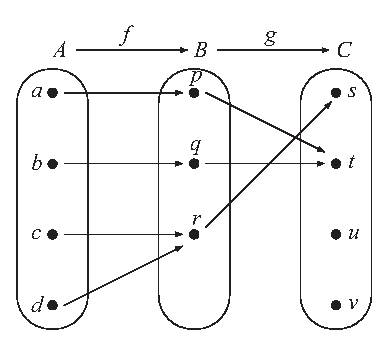
\includegraphics{figps-prev641.eps} 
\caption{Arrow Diagram Showing Two Functions} \label{fig:preview64}
\end{center}
\end{figure}
Notice that $a \in A$ and $ f(a) = p$.  Since $p \in B$, we can use the function $g$ and obtain 
$g(p) = t$.  This can be summarized as follows:
\[
g ( f(a) ) = g(p) = t.
\]
Using this process, determine $g ( f(b) )$, $g ( f(c) )$, and 
$g ( f(d) )$.  Then explain how we can now define a function from $A$ to $C$.

%Complete the following table.  For example,  if  $x = a$, then  $f( a ) = p$, and  $g( {f( a )} ) = g( p ) = t$.
%\begin{center}
%\begin{tabular}{ c  | c | c}
% $x$  &  $f( x )$  &  $g( {f( x )} )$ \\ \hline
% $a$  &                       &                                        \\ \hline
% $b$  &                       &                                        \\ \hline
% $c$  &                       &                                        \\ \hline
% $d$  &                       &                                        \\ \hline
%\end{tabular}
%\end{center}
%Explain how this table defines a function from  $A$  to  $C$.
\end{previewactivity}
\hbreak
%
\begin{previewactivity}[A New Function from Graphs] \label{PA:compositiongraphs} \hfill \\
Figure~\ref{fig:functioncomposition} shows the graphs of two real functions:  
$f\x \mathbb{R} \to \mathbb{R}$  and  $g\x \mathbb{R} \to \mathbb{R}$.  It also shows the graph of the line  $y = x$.
%\begin{figure}[h]
%\begin{center}
%\includegraphics[10.5cm,9.5cm]{figcomposition.bmp}
%\caption{Graph of $y = g( x )$ and  $y = f( x )$.} \label
%{fig:functioncomposition}
%\end{center}
%\end{figure}
\begin{figure}[h]
\begin{center}
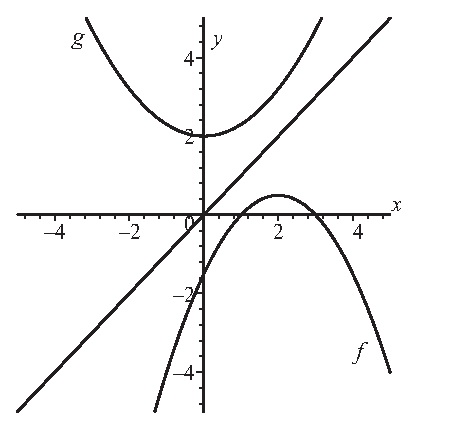
\includegraphics{figps-prev642.eps}
\caption{Graph of $y = g( x )$ and  $y = f( x )$} 
\label{fig:functioncomposition}
\end{center}
\end{figure}

%
\begin{enumerate}
\item We will first use  $x = 2$. \label{PA:compositiongraphs1}
\begin{enumerate}
  \item Draw the vertical line  $x = 2$  so that it intersects the graph of  $f$.  Label this point  $P$.  This point of intersection is  $( {2, f( 2 )} )$.  Although we could use the graph of  $f$  to approximate  $f( 2 )$, we will not do so here.
\label{PA:compositiongraphsa}

  \item Now draw a horizontal line through the point  $P$  until it intersects the  line  
$y = x$.  Call this point of intersection  $Q$.  What are the coordinates of the point  $Q$?  Each coordinate should be expressed in terms of the function  $f$\!.

  \item Next, draw a vertical line through the point  $Q$  until it intersects the graph of  
$g$.  Call this point of intersection  $R$.  What are the coordinates of the point  $R$  in terms of the functions  $f$  and  $g$?

  \item Finally, draw a horizontal line through the point  $R$  until it intersects the vertical line  $x = 2$ from Part~(\ref{PA:compositiongraphsa}).  Call this point of intersection  $S$.  What are the coordinates of the point  $S$  in terms of the functions  $f$  and  $g$.  Approximate the $y$-coordinate of the point  $S$?
\end{enumerate}

\item Repeat Part~(\ref{PA:compositiongraphs1}) starting with  $x = 3$.

\item Repeat Part~(\ref{PA:compositiongraphs1}) starting with  $x = 0$.

\item Explain how this process can be used to define a new function from  $\mathbb{R}$
to   $\mathbb{R}$.
\end{enumerate}

\end{previewactivity}
\hbreak
%
%\newpage
\begin{previewactivity}[Verbal Descriptions of Functions] \label{PA:verbaldescriptions} \hfill \\
The outputs of most real functions we have studied in previous mathematics courses have been determined by mathematical expressions.  In many cases, it is possible to use these expressions to give step-by-step verbal descriptions of how to compute the outputs.  For example, if
\[
f\x \mathbb{R} \to \mathbb{R}\text{  is defined by  }f( x ) = ( {3x + 2} )^3, 
\]
we could describe how to compute the outputs as follows:

\begin{center}
\begin{tabular}{| c | l | c|}
\hline
Step  &  \textbf{Verbal Description}  &  \textbf{Symbolic Result}  \\ \hline
1  &  Choose an input.	  &  $x$           \\  \hline
2  &  Multiply by 3.	  &  $3x$          \\  \hline
3  &  Add 2.	        &  $3x + 2$      \\  \hline
4  &  Cube the result.    &  $( {3x + 2} )^3 $  \\  \hline
\end{tabular}
\end{center}
Complete step-by-step verbal descriptions for each of the following functions.
\begin{enumerate}
\item $f\x \mathbb{R} \to \mathbb{R}$ by	$f( x ) = \sqrt {3x^2  + 2} $

\item $g\x \mathbb{R} \to \mathbb{R}$ by $g( x ) = \sin \! \left( {3x^2  + 2} \right)$

\item $h\x \mathbb{R} \to \mathbb{R}$ by	$h( x ) = e^{3x^2  + 2} $

%\item $F\x  \R \to \R$ by $F(x) = ( x^2 +3 )^3$.
%
%\item $G\x  \R \to \R$ by $G(x) = ln ( x^2 + 3 )$.
\end{enumerate}
\end{previewactivity}
\hbreak

\endinput

\begin{center}
\setlength{\unitlength}{0.5cm}
\begin{picture}(18,14)
\put(2,6.5){\oval(3,11)}
\put(8,6.5){\oval(3,11)}
\put(14,6.5){\oval(3,11)}

\put(2,2){\circle*{.5}}
\put(2,5){\circle*{.5}}
\put(2,8){\circle*{.5}}
\put(2,11){\circle*{.5}}

\put(8,5){\circle*{.5}}
\put(8,8){\circle*{.5}}
\put(8,11){\circle*{.5}}

\put(14,2){\circle*{.5}}
\put(14,5){\circle*{.5}}
\put(14,8){\circle*{.5}}
\put(14,11){\circle*{.5}}

\put(1.1,11){$a$}
\put(1.1,8){$b$}
\put(1.1,5){$c$}
\put(1.1,2){$d$}

\put(8,11.5){$p$}
\put(8,8.5){$q$}
\put(8,5.5){$r$}

\put(14.5,11){$s$}
\put(14.5,8){$t$}
\put(14.5,5){$u$}
\put(14.5,2){$v$}

\put(2,12.5){$A$}
\put(8,12.5){$B$}
\put(14,12.5){$C$}


\put(3,12.8){\vector(1,0){4.7}}
\put(9,12.8){\vector(1,0){4.7}}

\put(5,13.2){$f$}
\put(11,13.2){$g$}

\put(2.5,11){\vector(1,0){5}}
\put(2.5,8){\vector(1,0){5}}
\put(2.5,5){\vector(1,0){5}}
\put(2.5,2){\vector(2,1){5}}

\put(8.5,11){\vector(2,-1){5}}
\put(8.5,8){\vector(1,0){5}}
\put(8.5,5.3){\vector(1,1){5.3}}

\end{picture}
\end{center}
